\myslide{Parser - Autovervollständigung}
{
  \begin{itemgroup}{Übersicht}
    \item Die Parser waren sehr unübersichtlich strukturiert
    \item Pro Ausdruck und Typ wurde ein eigenes \glqq non terminal\grqq eingeführt
    \item Zusätzlich ein eigenes \glqq error non terminal\grqq, welches sich um
          die eingeführte Fehlerbehandlung kümmert
    \item Jedem geparsten Ausdruck wird seine Source Code Position mitgegeben, um
          Fehler anzeigen zu können und, um den Source Code durch die Outline
          markieren zu lassen
    \item Eine automatische Vervollständigung wurde eingeführt, um vom Benutzer
          eingegebene, noch unvollständige Ausdrücke per Mausklick zu vervollständigen
    \item Fehlermeldungen, die mehrere Stellen betreffen, wurden eingeführt
          (z.B. keine disjunkten Mengen bei den Identifiern) 
  \end{itemgroup}
}

\myslide{Parser - Autovervollständigung}
{
  Gibt der Anwender \glqq \ExprInfixOperation{+}{1}{\KeyLet\ \ExprIdentifier{x} =}\grqq\ 
  ein, wird der Teil \glqq \KeyLet\ \ExprIdentifier{x} =\grqq\ hervorgehoben und der Tooltip
  verrät dem Anwender, dass er noch den Ausdruck \glqq $e_1$\ \KeyIn\ $e_2$\grqq\ eingeben muss,
  um \glqq{\bf Let}\grqq\ zu vervollständigen. Durch einen Mausklick auf das Symbol wird der
  fehlende Code ergänzt.
  \begin{center}
    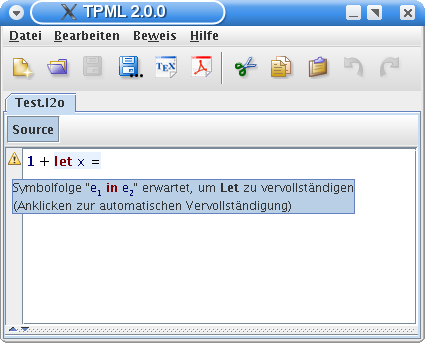
\includegraphics[height=10cm]{images/parser_auto.png}
  \end{center}
}

\myslide{Parser - Fehlermeldungen}
{
  Gibt der Anwender einen Ausdruck ein, der laut Theorie nicht zulässig ist, werden die entsprechenden
  Stellen rot unterstrichen. In diesem Beispiel ist ein Objekt mit Attributen mit dem gleichen Namen
  laut Theorie nicht erlaubt.
  \begin{center}
    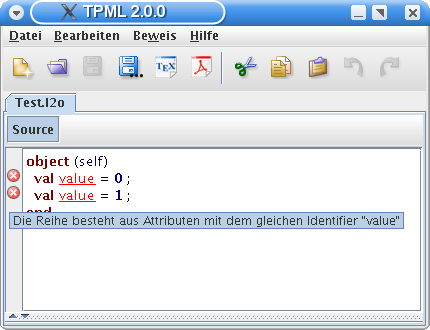
\includegraphics[height=10cm]{images/parser_error.png}
  \end{center}
}

\myslide{Parser - Korrekturen}
{
  Gibt der Anwender einen Ausdruck ein, der laut Theorie nicht zulässig ist, eine Korrektur aber durch
  einfaches Umbenennen möglich ist, wird dies dem Anwender vorgeschlagen. Klickt er auf das blaue Icon,
  werden die entsprechenden Identifier umbenannt.
  \begin{center}
    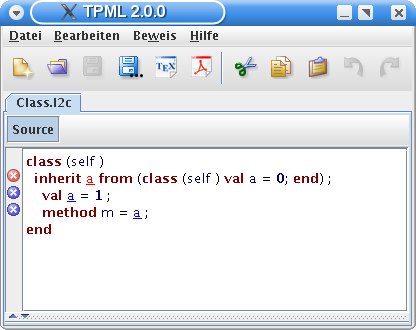
\includegraphics[height=10cm]{images/parser_rename.png}
  \end{center}
}